\documentclass{article}

% if you need to pass options to natbib, use, e.g.:
%     \PassOptionsToPackage{numbers, compress}{natbib}
% before loading neurips_2020

% ready for submission
% \usepackage{neurips_2020}

% to compile a preprint version, e.g., for submission to arXiv, add add the
% [preprint] option:
%     \usepackage[preprint]{neurips_2020}

% to compile a camera-ready version, add the [final] option, e.g.:
     \usepackage[final]{neurips_2020}

% to avoid loading the natbib package, add option nonatbib:
%     \usepackage[nonatbib]{neurips_2020}

\usepackage[utf8]{inputenc} % allow utf-8 input
\usepackage[T1]{fontenc}    % use 8-bit T1 fonts
\usepackage{hyperref}       % hyperlinks
\usepackage{url}            % simple URL typesetting
\usepackage{booktabs}       % professional-quality tables
\usepackage{amsfonts}       % blackboard math symbols
\usepackage{nicefrac}       % compact symbols for 1/2, etc.
\usepackage{microtype}      % microtypography
\usepackage{graphicx}
\usepackage{float}

\title{AI Project 1: Drug Molecular Toxicity Prediction}

% The \author macro works with any number of authors. There are two commands
% used to separate the names and addresses of multiple authors: \And and \AND.
%
% Using \And between authors leaves it to LaTeX to determine where to break the
% lines. Using \AND forces a line break at that point. So, if LaTeX puts 3 of 4
% authors names on the first line, and the last on the second line, try using
% \AND instead of \And before the third author name.

\author{
MATSUNAGA TAKEHIRO \\
518030990028\\
Department of Computer Science\\
Shanghai Jiao Tong University\\
\texttt{matsunagatakehiro@sjtu.edu.cn} \\
}


\begin{document}

\maketitle

\begin{abstract}
 I develop some models to solve a problem whether a chemical is toxic or not. In this project I use 2 long short-term memory(LSTM) and a complex CNN based on LeNet-5. Through several experiment I found that the complex neural network is most accurate among these model.
\end{abstract}

\section{Introduction}
This project is the group project of CS410 Artificial Intelligence 2020 Fall in Shanghai Jiao Tong University named Drug Molecular Toxicity Prediction. The main purpose is to use a neural network model taking chemical structure as input, to output the prediction of whether it is toxic. In this project I use one hot format of SMILE structure which is processed from original chemical structure. The one hot format of SMILES is a 2D {0,1} matrix, where each column represents a symbol in the SMILES notation of the current molecule, and each row is one ASCII character appeared in the dataset’s SMILES dictionary.
% The authors develop two different neural network models, which are Deep Fully Connected Neural Networks with Merge-and-Run Mappings(DMRNets) and LSTM in their attempts to achieve this goal.


\section{Methods}
\subsection{Input Data analysis}
First, I analyzed the input data in this project.Through the interface that demo provide me, I could directly get the processed input in the model. By calling the print function to print input shape to screen, I found that input shpae is (?, 73, 398), which means each size of chemical is 73$\times$398. 

\subsection{Complex Convolutional Neural Networks}
Based on LeNet-5 which is given in the demo, I optimize that model by using batch normalization, droupout and so on. 
\subsubsection{CNN}
convolutional neural network (CNNt) is a class of neural networks, most commonly applied to analyzing image. CNN has feature kernel that to determine whether each part of the image with the kernel size has the feature, if it is, it may return a higher value. When running the CNN, the input tensor with shape $number*height*width*input channel$ will be processed into $number*height*width*feature channel$ if user fill some blank and keep image size same.

\subsubsection{LeNet-5}
LeNet-5 is a simple but usefull CNN which is widely used in image processing. The original LeNet-5 consists of seven layers: 2 convolution layer, 2 pooling layer and 3 full connection layer. The input data will first processed by Layer 1 convolution, that has 5$\times$5 kernel. Through the convolution it will increase the data channel. The pooling is use to reduce its size, and outstand feature value in pooling kernel. When the size is small enough--in LeNet-5 run the function after 2 convolution and pooling-- model run the full connection and shrink node to label size by using 3 layers. The Figure \ref{LeNet} show the structure of LeNet-5.
\begin{figure}[h]
  \centering
  \fbox{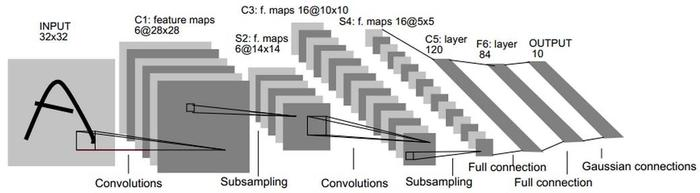
\includegraphics[width=14cm, height=4cm]{LeNet-5.png}}
  \caption{Structure of LeNet-5}
  \label{LeNet}
\end{figure} 

\subsubsection{Complex CNN}
I first think that whether I can build an improved model based on the demo, which is LeNet-5 inside. So I try to add some layers to test whether the AUC can increase.

Though my effort I get a bit powerful model than vanilla LeNet-5, which is add batch normalization after each convolution and dense layer, so that the regularization can work on the processed data. After each pooling, I use dropout to make some noise in order to enhance the model. The overview of Complex CNN structure is show in Figure \ref{Complex CNN}, which directly display which layer the model contains.
 
\begin{figure}
	\centering
	\fbox{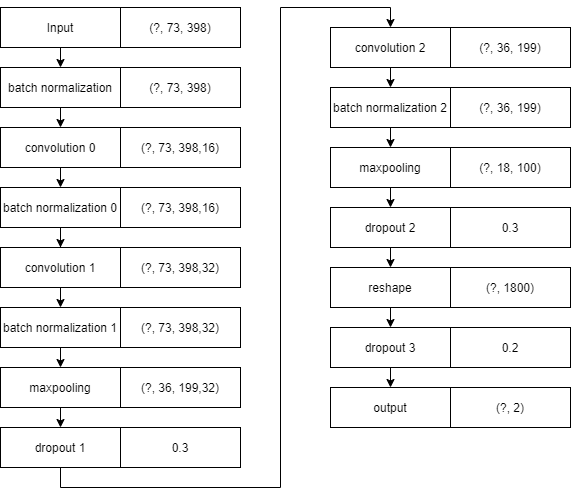
\includegraphics[width=14cm, height=11cm]{complex-cnn.png}}
	\caption{Structure of complex-cnn}
	\label{Complex CNN}
\end{figure} 




\subsection{CNN + LSTM}
\subsubsection{Model Overview}
Long short-term memory(LSTM) is a type of recurrent neural network (RNN) architecture,which is one of the most useful RNN.  Before LSTM, let's first talk about RNN. As brain can understand articles based on knowledge that people have learnt before, some parameters in RNN can be derived from forward node, this was what traditional neural networks could not achieve. Traditional RNN could not store what it learned from forward node for a dragged time period, since every cell of RNN will process both input and derived information in activation function, but LSTM solved this problem.


A common LSTM unit is composed of a cell and 3 gates. The cell stores values over time intervals as cell states, and the 3 gates’ main job is to regulate the flow of information into and out of the cell. Specifically, forget gate decides which information to forget, input gate decides to update which value of cell states and update cell states, and at last, the output gate output filtered cell states. To put it in an abstract high-level view, what LSTM do is using past context as reference to predict the output.Beside forward outputs, another data are derived from forward nodes in LSTM network. The increasing data will only interact with a few data that processed in cell, which means it will keep the knowledge that it learned for a long time.

\begin{figure}[h]
  \centering
  \fbox{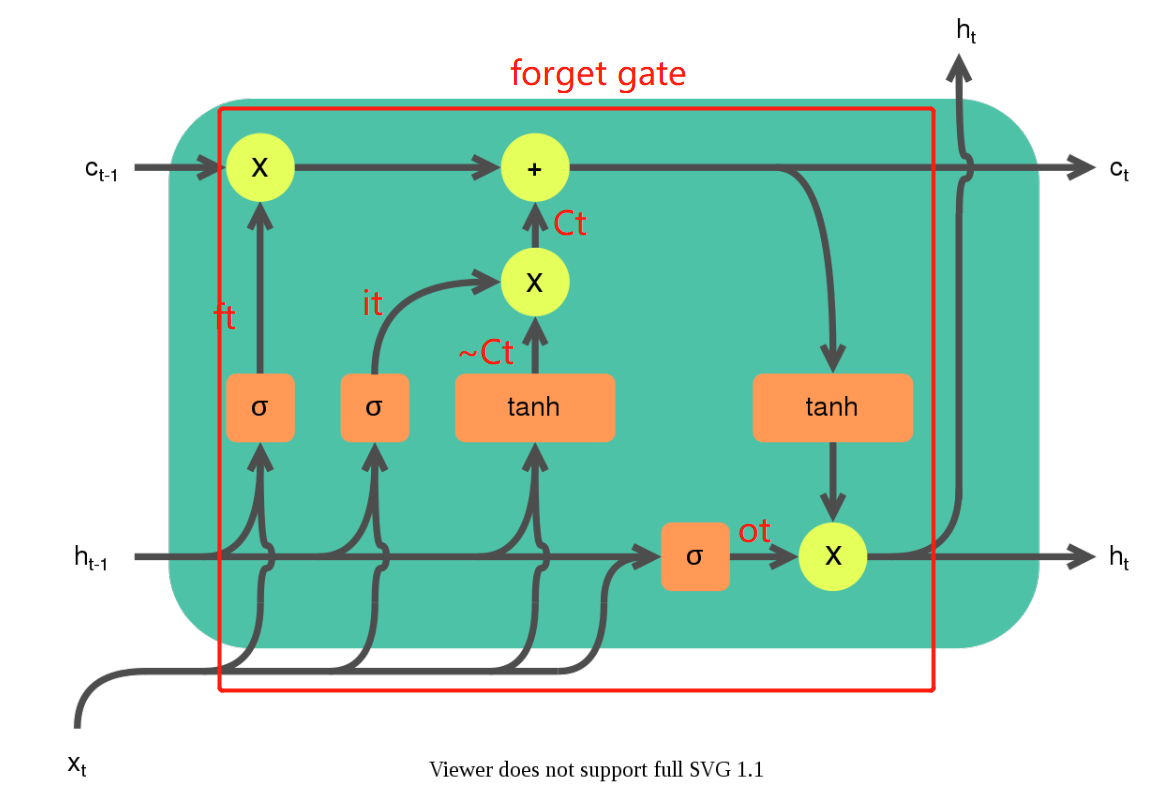
\includegraphics[width=9cm, height=5.6cm]{lstm.png}}
  \caption{Structure of LSTM Cell}
\end{figure} 


Here are each step in the forget gate of LSTM cell:
\begin{itemize}
\item step1: $f_t = \sigma(W_f[h_{t-1}, x_t] + b_f)$
\item step2: $i_t = \sigma(W_i[h_{t-1}, x_t] + b_i)$,  $\widetilde{C} = tanh(W_C[h_{t-1}, xt] + b_C)$
\item step3: $o_t=\sigma(W_o[h_{t-1}, x_t] + b_o)$
\item step4: $C_t = f_t*C_{t-1} + i_t*\widetilde{C}$
\item step5: $h_t=o_t*tanh(C_t)$
\end{itemize}

\subsubsection{Contribute idea}
The reason why I use CNN first is that the input size is too huge for my computer to caluculate directly. So CNN and pooling is necessary for reduce the size. When passing the CNN layer, the size of each piece of data is $18*50*32$. So I can run the processed input on LSTM, which can keep some forward information. The Figure \ref{LSTMstruct} shows the structure of the model.

\begin{figure}[h]
	\centering
	\fbox{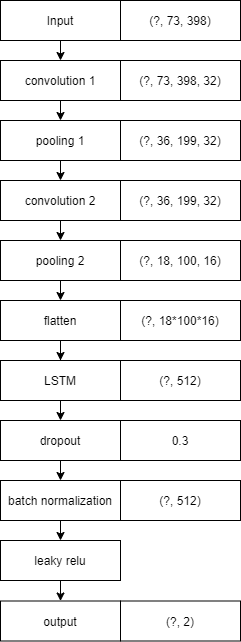
\includegraphics[width=14cm, height=8.5cm]{CNN+LSTM.png}}
	\caption{Structure of CNN+LSTM}
	\label{LSTMstruct}
\end{figure} 

\subsection{CNN+BiLSTM}
\subsubsection{Model Overview}
Bidirectional Long short-term memory(BiLSTM) is a variant of LSTM, biLSTM train 2 instead of 1 LSTMs on input sequence, the first on the input sequence, and the second on a reversed copy of the input sequence. In other words, it connects two hidden layers of opposite directions to the same output, this generally provide additional context to the network, thus results in better training results. And each LSTM in BiLSTM structure will produce a output which will provide the other one as future prediction. 

\begin{figure}[h]
	\centering
	\fbox{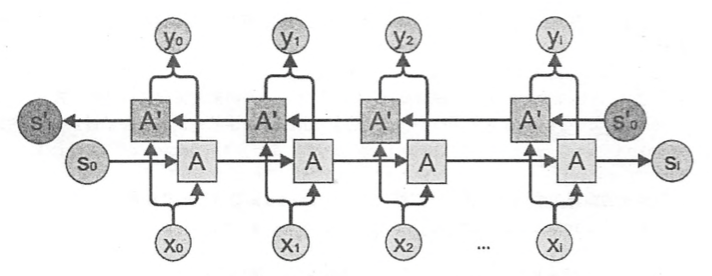
\includegraphics[width=12cm, height=5cm]{BiLSTM.png}}
	\caption{Structure of BiLSTM}
\end{figure} 

Like the structure of CNN+LSTM, I change the LSTM layer into the Bidirectional LSTM layer. 

\section{Experiments and Analysis}
\subsection{Environment}
In this project, TensorFlow-gpu 1.15.0 is used as deep learning library, Pandas is used to input data and Numpy is used through mathmatical calculation.

The platform I train and test the model is on my own local machine, whose CPU is i5-8500, GPU is GTX 1060-16G, and RAM size is 24G.

\subsection{Training}
Complex CNN has the most high AUC value among the model I use. The final AUC of weight I got is 0.826. The curve is displayed in Figure \ref{CNN}.

\begin{figure}[h]
	\centering
	\fbox{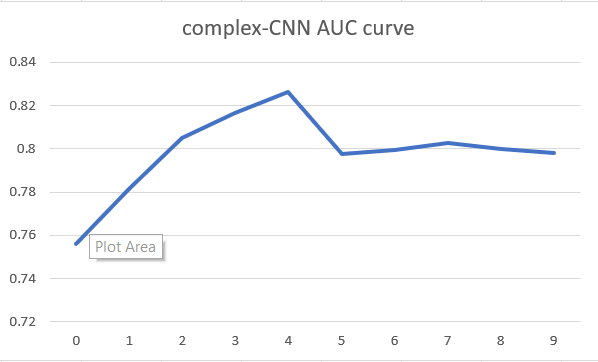
\includegraphics[width=12cm, height=7cm]{complex-cnn-auc.png}}
	\caption{AUC curve of Complex CNN}
	\label{CNN}
\end{figure} 

The hightest AUC value of CNN+LSTM is 0.784. The curve is displayed in Figure \ref{CNN+LSTM}.

\begin{figure}[h]
	\centering
	\fbox{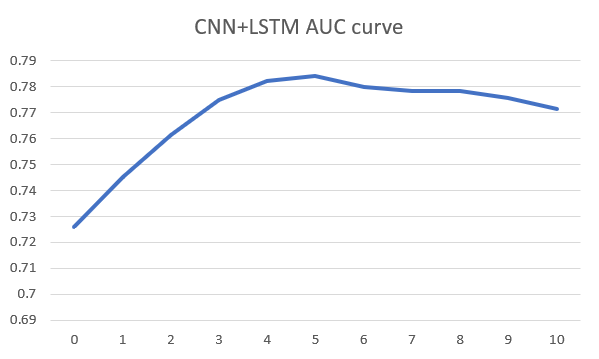
\includegraphics[width=12cm, height=7cm]{CNN+LSTM-auc.png}}
	\caption{AUC curve of CNN+LSTM}
	\label{CNN+LSTM}
\end{figure} 

The hightest AUC value of CNN+LSTM I got is 0.803. The curve is displayed in Figure \ref{CNN+BiLSTM}.
\begin{figure}[h]
	\centering
	\fbox{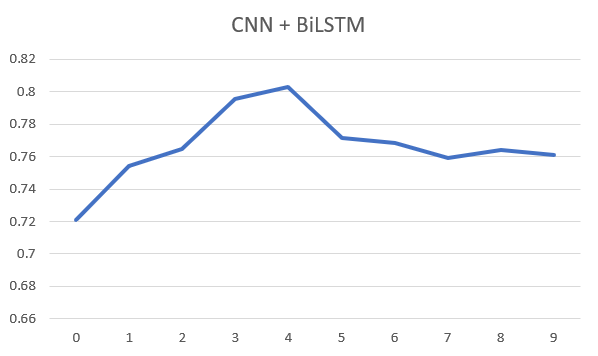
\includegraphics[width=12cm, height=7cm]{CNN+BiLSTM-auc.png}}
	\caption{AUC curve of CNN+BiLSTM}
	\label{CNN+BiLSTM}
\end{figure} 

\section{Conclusion}
The performances of 3 models are listed in Table \ref{table 1}. As shown in the table, the Complex CNN has the most powerful performance in these models. The AUC of Complex CNN can get 0.826 and its AUC test result in Kaggle is about 0.858, which shows in Figure \ref{final result}. 
\begin{table} [h]
  \caption{Performance of different models}
  \label{table 1}
  \centering
  \begin{tabular}{c|c|c}
    \toprule
   	Model   	& \quad final AUC \quad &\quad test result \quad \\
    \midrule 
	Complex-CNN & 0.826 & 0.858\\
	CNN + LSTM  & 0.784 & 0.842\\
	CNN + BiLSTM& 0.803 & 0.855\\
    \bottomrule
  \end{tabular}
\end{table}

\begin{figure}[h]
	\centering
	\fbox{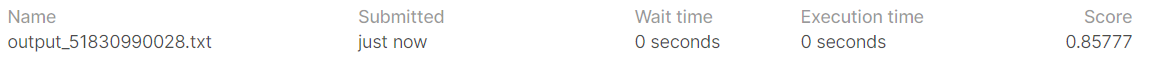
\includegraphics[width=15cm, height=0.8cm]{complex-cnn-result.png}}
	\caption{test result of project 1}
	\label{final result}
\end{figure} 




\section*{References}
[1] Sepp Hochreiter. Long Short-Term Memory. 

[2] Alex Graves, Jürgen Schmidhuber. Framewise phoneme classification with bidirectional LSTM and other neural network architectures. 
\end{document}
